\documentclass{article}
\usepackage{pdfpages} 
\usepackage[utf8]{vietnam}
\usepackage{graphicx}
\usepackage{amsmath}
\usepackage{float}
\usepackage{hyperref}
\usepackage{listings}
\usepackage{color}
\usepackage{indentfirst}
\usepackage{cases}
\usepackage{tabularx}

\definecolor{dkgreen}{rgb}{0,0.6,0}
\definecolor{gray}{rgb}{0.5,0.5,0.5}
\definecolor{mauve}{rgb}{0.58,0,0.82}

\lstset{frame=tb,
  language=Java,
  aboveskip=3mm,
  belowskip=3mm,
  showstringspaces=false,
  columns=flexible,
  basicstyle={\small\ttfamily},
  numbers=none,
  numberstyle=\tiny\color{gray},
  keywordstyle=\color{blue},
  commentstyle=\color{dkgreen},
  stringstyle=\color{mauve},
  breaklines=true,
  breakatwhitespace=true,
  tabsize=3
}

\definecolor{codegreen}{rgb}{0,0.6,0}
\definecolor{codegray}{rgb}{0.5,0.5,0.5}
\definecolor{codepurple}{rgb}{0.58,0,0.82}
\definecolor{backcolour}{rgb}{0.95,0.95,0.92}

\lstdefinestyle{mystyle_code}{
    backgroundcolor=\color{backcolour},   
    commentstyle=\color{codegreen},
    keywordstyle=\color{magenta},
    numberstyle=\tiny\color{codegray},
    stringstyle=\color{codepurple},
    basicstyle=\ttfamily\footnotesize,
    breakatwhitespace=false,         
    breaklines=true,                 
    captionpos=b,                    
    keepspaces=true,                 
    numbers=left,                    
    numbersep=5pt,                  
    showspaces=false,                
    showstringspaces=false,
    showtabs=false,                  
    tabsize=2
}


\begin{document}

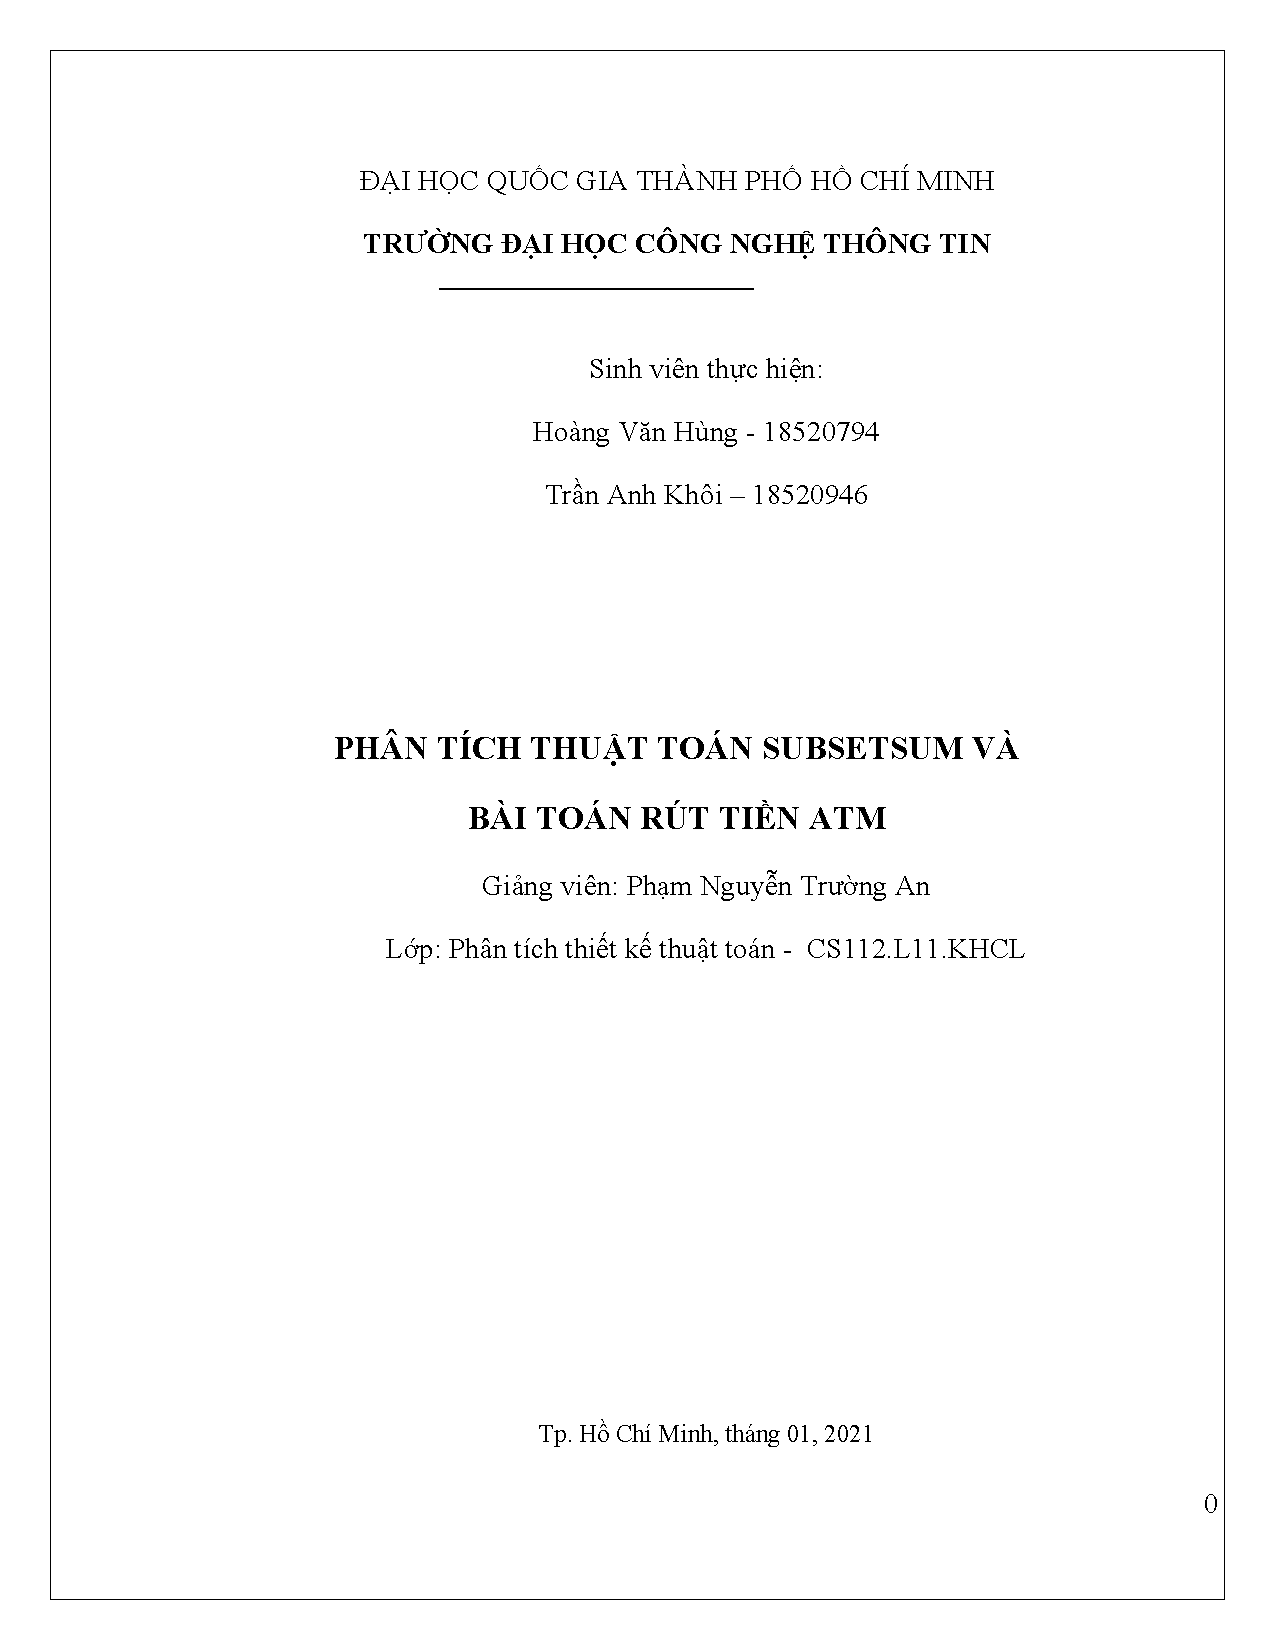
\includepdf[page={1}, scale=0.9]{img/final.pdf}

\tableofcontents{}
\newpage
\section{Giới thiệu bài toán: }
\subsection{Mục tiêu và giới thiệu bài toán}
Phân tích thiết kế và đánh giá thuật toán là một trong những chìa khóa để xác định hiệu suất của hệ thống khi giải các bài toán máy tính. Có nhiều vấn đề với các giải pháp đưa ra chỉ ở mức chấp nhận được và việc tính toán chỉ cho phép chấp nhận một sai số nhất định.
Về giải bài toán này có nhiều phương pháp giải: Phương pháp quy hoạch động, phương pháp tham lam, phương pháp tiếp cận ...
Trong đồ án này chúng tôi lựa chọn Bài toán rút tiền ATM, một bài toán trong lĩnh vực tối ưu hóa tổ hợp. Dùng phương pháp quy hoạch động để giải bài toán.
\subsection{Lịch sử}
Subset Sum là một bài toán tối ưu hóa cổ điển, nó là  một ví dụ về NP-hard problem, có thể phù hợp với lập trình động, mang lại thời gian chạy đa thức nếu số đầu vào tương đối nhỏ. Về mặt hình thức, cho trước một tập hợp S gồm n số nguyên dương và một số nguyên đích t, bài toán SubsetSum là quyết định xem có một tập hợp con của S tổng bằng t hay không. Với lập trình động thì thời gian chạy của nó là $O(nt)$. Subset sum được ra đời năm 1982..
\subsection{Ứng dụng}
Một tình huống thực tế khác đó là bài toán rút tiền ATM. ATM đang dần trở thành một phần thiết yếu của cuộc sống khi các doanh nghiệp đang chuyển hoàn toàn sang việc trả lương thông qua tài khoản ngân hàng. Một trong những tác vụ chính của ATM là tính toán để có thể lấy ra một lượng tiền chính xác như yêu cầu vào giao cho người sử dụng.
\section{Phân tích và thiết kế }
\paragraph{Sử dụng phương pháp quy hoạch động }
Phương pháp quy hoạch động dùng để giải bài toán tối ưu có bản chất đệ quy, tức là việc tìm phương án tối ưu cho bài toán đó có thể đưa về tìm phương án tối ưu của một số hữu hạn các bài toán con. Đối với nhiều thuật toán đệ quy chúng ta đã tìm hiểu, nguyên lý chia để trị (divide and conquer) thường đóng vai trò chủ đạo trong việc thiết kế thuật toán. Để giải quyết một bài toán lớn, ta chia nó làm nhiều bài toán con cùng dạng với nó để có thể giải quyết độc lập. Trong phương pháp quy hoạch động, nguyên lý này càng được thể hiện rõ: 
Khi không biết cần phải giải quyết những bài toán con nào, ta sẽ đi giải quyết tất cả các bài toán con và lưu trữ những lời giải hay đáp số của chúng với mục đích sử dụng lại theo một sự phối hợp nào đó để giải quyết những bài toán tổng quát hơn. Đó chính là điểm khác nhau giữa Quy hoạch động và phép phân giải đệ quy và cũng là nội dung phương pháp quy hoạch động: 
Phép phân giải đệ quy bắt đầu từ bài toán lớn phân rã thành nhiều bài toán con và đi giải từng bài toán con đó. Việc giải từng bài toán con lại đưa về phép phân rã tiếp thành nhiều bài toán nhỏ hơn và lại đi giải tiếp bài toán nhỏ hơn đó bất kể nó đã được giải hay chưa. 
Quy hoạch động bắt đầu từ việc giải tất cả các bài toán nhỏ nhất (bài toán cơ sở) để từ đó từng bước giải quyết những bài toán lớn hơn, cho tới khi giải được bài toán lớn nhất (bài toán ban đầu). 
\subsection{Cách giải}
Gọi S[i,t] là số lượng tờ tiền cần trả khách (cách trả cần ít tờ tiền nhất) có sử dụng i loại tờ tiền (1, 2, 3,…, n) cho số tiền T.
Giá trị cuối cùng S[n,T] là kết quả của cách thanh toán; dùng n loại tờ tiền (1, 2, 3, …, n) cho số tiền T.
\subsection{Mã giả}
\lstset{style=mystyle_code}
\begin{lstlisting}[language=Python, caption=Mã giả subset sum, mathescape=true]
SubsetSum(X[1,2, ... ,n],T):  
    	$S[0,0] \xleftarrow{} True$ 
        for $ t \xleftarrow{} to$ T
        		$S[0,t]\xleftarrow{}False$  
        for $ i \xleftarrow{} 1 to$ n
        		$S[i,0]\xleftarrow{} True$   
        for $ t \xleftarrow{} 1$ to X[i]-1  
          		$S[i,t]\xleftarrow{}S[i-1,t]$    
          		avoid the case t-X[i]<0
        for $ t \xleftarrow{}X[i]$ to T 
         		$S[i,t]\xleftarrow{}S[i-1,t] or S[i-1,t-X[i]]$
return $S[n,T]$
\end{lstlisting}
\paragraph{Giải thích mã giả:}
Chúng ta sẽ tạo một mảng 2 chiều có kích thước (arr.size () + 1) * (target + 1) kiểu boolean. Trạng thái S[i,t] sẽ đúng nếu tồn tại một tập hợp con các phần tử từ X[0… .i] với giá trị tổng = 't' : 
Nếu phần tử hiện tại có giá trị lớn hơn “tổng hiện tại”, chép giá trị cho các trường hợp trước.
Và nếu tổng hiện tại lớn hơn phần tử thứ i, sẽ xem xét  liệu có bất kì trường hợp nào trước đó đã có tổng = ‘t’ hoặc bất kì trạng thái nào có giá trị ‘t – X[i]’. 
\subsection{Mã nguồn}
\lstinputlisting[language=Python]{source_code/subset.py}
\subsection{Phát sinh Input/Output}
    \paragraph{Input}
Input là một mảng các tờ tiền có trong mấy và số tiền khách hàng cần rút
    \paragraph{Output}
Là những tờ tiền máy trả cho khách hàng 
\emph{Ví dụ}\\
\begin{tabular}{|p{2.3in}|p{0.8in}|p{1.8in}|} \hline 
Tiền trong máy ATM & Tiền muốn rút & Tiền trả \\ \hline 
[500.000,200.000,100.000,50.000,\newline 20.000] & 600.000 & [500.000,100.000] \\ \hline 
[500.000,500.00,100.000,200.000,\newline 50.000,20.000] & 820.000 & [500.000,100.000,200.000,\newline 20.000] \\ \hline 
\end{tabular}
\subsubsection{Mã nguồn phát sinh Input/Output}
\lstinputlisting[language=Python]{source_code/input_output_generate.py}

\subsubsection{Kiểm tra tính đúng đắn của Mã nguồn}
\lstinputlisting[language=Python]{source_code/source.py}
\subsection{Phân tích độ phức tạp}
Thời gian tính toán của thuật toán SubsetSum có thể được quy về thời gian cập nhật các phần tử của mảng S[n,T]. Vì mỗi phần tử của mảng được cập nhật trong thời gian $O(1)$, thời gian tính toán của thuật toán là O(nT) với n là số phần tử của mảng.
Độ phức tạp bộ nhớ là $O(nT)$ với bộ nhớ của mảng 2 chiều là n*T.
\subsection{Phân tích thực nghiệm}
\subsubsection{Phát sinh dữ liệu để phân tích độ phức tạp}
Mảng n chứa các số nguyên được tạo ngẫu nhiên từ 1- 50 phần tử.
Giá trị T là giá trị tổng mong muốn được tạo ngẫu nhiên trong khoảng 0-1000.
\subsubsection{Bảng thực nghiệm độ phức tạp: }

\begin{itemize}
    \item Tính giá trị của nT theo các độ phức tạp
    \begin{table}[H]
\scalebox{0.8}{\begin{tabular}{|l|l|l|l|l|l|l|l|l|l|l|l|l|l|}
\centering
\toprule
    & $nT$ & $T(nT)$ & $lg(nT)$ & $sqrt(nT)$ & $(nT)lg(nT)$ & $(nT)^2$ & $(nT)^3$ & $2^(nT)$ & $(nT)!$\\
\midrule
\hline
    0     & 60    & 332   & 5.91E+00 & 7.75E+00 & 3.54E+02 & 3.60E+03 & 2.16E+05 & 1.15E+24 & 8.32E+87 \\
    \hline
    1     & 123   & 886   & 6.94E+00 & 1.11E+01 & 8.54E+02 & 1.51E+04 & 1.86E+06 & 1.06E+43 & 1.21E+211 \\
    \hline
    2     & 222   & 2749  & 7.79E+00 & 1.49E+01 & 1.73E+03 & 4.93E+04 & 1.09E+07 & 6.74E+72 & 1.12050E+427 \\
    \hline
    3     & 396   & 2089  & 8.63E+00 & 1.99E+01 & 3.42E+03 & 1.57E+05 & 6.21E+07 & 1.61E+125 & 2.53926E+859 \\
    \hline
    4     & 516   & 5627  & 9.01E+00 & 2.27E+01 & 4.65E+03 & 2.66E+05 & 1.37E+08 & 2.15E+161 & 2.43656E+1178 \\
    \hline
    5     & 855   & 10266 & 9.74E+00 & 2.92E+01 & 8.33E+03 & 7.31E+05 & 6.25E+08 & 2.40E+263 & 2.36788E+2138 \\
    \hline
    6     & 1102  & 7909  & 1.01E+01 & 3.32E+01 & 1.11E+04 & 1.21E+06 & 1.34E+09 & 5.43319E+332 & 6.48353E+2876 \\
    \hline
    7     & 1166  & 8517  & 1.02E+01 & 3.41E+01 & 1.19E+04 & 1.36E+06 & 1.59E+09 & 1.00224E+352 & 2.06830E+3072 \\
    \hline
    8     & 1872  & 21486 & 1.09E+01 & 4.33E+01 & 2.03E+04 & 3.50E+06 & 6.56E+09 & 3.37405E+564 & 6.20201E+5315 \\
    \hline
    9     & 2538  & 19385 & 1.13E+01 & 5.04E+01 & 2.87E+04 & 6.44E+06 & 1.63E+10 & 1.03306E+765 & 2.89521E+7541 \\
    \hline
    10    & 3880  & 39002 & 1.19E+01 & 6.23E+01 & 4.63E+04 & 1.51E+07 & 5.84E+10 & 9.91706E+1168 & 6.28088E+12242 \\
    \hline
    11    & 4060  & 43748 & 1.20E+01 & 6.37E+01 & 4.87E+04 & 1.65E+07 & 6.69E+10 & 1.51978E+1223 & 3.83231E+12890 \\
    \hline
    12    & 4544  & 53008 & 1.21E+01 & 6.74E+01 & 5.52E+04 & 2.06E+07 & 9.38E+10 & 7.59102E+1368 & 1.56109E+14649 \\
    \hline
    13    & 5863  & 67254 & 1.25E+01 & 7.66E+01 & 7.34E+04 & 3.44E+07 & 2.02E+11 & 8.68689E+1765 & 3.17357E+19549 \\
    \hline
    14    & 6030  & 65887 & 1.26E+01 & 7.77E+01 & 7.57E+04 & 3.64E+07 & 2.19E+11 & 1.62507E+1816 & 6.41092E+20179 \\
    \hline
    15    & 6272  & 65924 & 1.26E+01 & 7.92E+01 & 7.91E+04 & 3.93E+07 & 2.47E+11 & 1.14850E+1889 & 5.41441E+21096 \\
    \hline
    16    & 6305  & 71988 & 1.26E+01 & 7.94E+01 & 7.96E+04 & 3.98E+07 & 2.51E+11 & 9.86558E+1898 & 1.22103E+21222 \\
    \hline
    17    & 6462  & 72223 & 1.27E+01 & 8.04E+01 & 8.18E+04 & 4.18E+07 & 2.70E+11 & 1.80232E+1946 & 3.05204E+21819 \\
    \hline
    18    & 6512  & 71190 & 1.27E+01 & 8.07E+01 & 8.25E+04 & 4.24E+07 & 2.76E+11 & 2.02923E+1961 & 1.22576E+22010 \\
    \hline
    19    & 6764  & 68300 & 1.27E+01 & 8.22E+01 & 8.61E+04 & 4.58E+07 & 3.09E+11 & 1.46855E+2037 & 1.75171E+22973 \\
    \hline
    20    & 6838  & 78635 & 1.27E+01 & 8.27E+01 & 8.71E+04 & 4.68E+07 & 3.20E+11 & 2.77402E+2059 & 7.17883E+23256 \\
    \hline
    21    & 6923  & 82670 & 1.28E+01 & 8.32E+01 & 8.83E+04 & 4.79E+07 & 3.32E+11 & 1.07314E+2085 & 1.13815E+23583 \\
    \hline
    22    & 6996  & 70177 & 1.28E+01 & 8.36E+01 & 8.94E+04 & 4.89E+07 & 3.42E+11 & 1.01356E+2107 & 3.68579E+23863 \\
    \hline
    23    & 7150  & 83611 & 1.28E+01 & 8.46E+01 & 9.15E+04 & 5.11E+07 & 3.66E+11 & 2.31456E+2153 & 2.56390E+24456 \\
    \hline
    24    & 7527  & 86262 & 1.29E+01 & 8.68E+01 & 9.69E+04 & 5.67E+07 & 4.26E+11 & 7.12487E+2266 & 5.44505E+25913 \\
    \hline
    25    & 8892  & 103147 & 1.31E+01 & 9.43E+01 & 1.17E+05 & 7.91E+07 & 7.03E+11 & 5.73748E+2677 & 1.34960E+31256 \\
    \hline
    26    & 8932  & 105112 & 1.31E+01 & 9.45E+01 & 1.17E+05 & 7.98E+07 & 7.13E+11 & 6.30842E+2689 & 1.34950E+31414 \\
    \hline
    27    & 9443  & 106710 & 1.32E+01 & 9.72E+01 & 1.25E+05 & 8.92E+07 & 8.42E+11 & 4.22911E+2843 & 2.02996E+33439 \\
    \hline
    28    & 9594  & 108673 & 1.32E+01 & 9.79E+01 & 1.27E+05 & 9.20E+07 & 8.83E+11 & 1.20719E+2889 & 1.18601E+34040 \\
    \hline
    29    & 9720  & 111475 & 1.32E+01 & 9.86E+01 & 1.29E+05 & 9.45E+07 & 9.18E+11 & 1.02697E+2927 & 1.46776E+34542 \\
    \hline
    30    & 9918  & 114101 & 1.33E+01 & 9.96E+01 & 1.32E+05 & 9.84E+07 & 9.76E+11 & 4.12569E+2986 & 3.97097E+35332 \\
    \hline
    31    & 11328 & 131256 & 1.35E+01 & 1.06E+02 & 1.53E+05 & 1.28E+08 & 1.45E+12 & 1.16893E+3411 & 1.53527E+41009 \\
    \hline
    32    & 11725 & 131936 & 1.35E+01 & 1.08E+02 & 1.58E+05 & 1.37E+08 & 1.61E+12 & 3.77310E+3530 & 4.77564E+42621 \\
    \hline
    33    & 11808 & 137690 & 1.35E+01 & 1.09E+02 & 1.60E+05 & 1.39E+08 & 1.65E+12 & 3.64912E+3555 & 3.50118E+42959 \\
    \hline
    34    & 12768 & 150534 & 1.36E+01 & 1.13E+02 & 1.74E+05 & 1.63E+08 & 2.08E+12 & 3.55618E+3844 & 2.27543E+46885 \\
    \hline
    35    & 14784 & 170992 & 1.39E+01 & 1.22E+02 & 2.05E+05 & 2.19E+08 & 3.23E+12 & 2.67581E+4451 & 1.19843E+55229 \\
    \hline
    36    & 16192 & 187075 & 1.40E+01 & 1.27E+02 & 2.26E+05 & 2.62E+08 & 4.25E+12 & 1.89535E+4875 & 2.51830E+61128 \\
    \hline
    37    & 16659 & 190334 & 1.40E+01 & 1.29E+02 & 2.34E+05 & 2.78E+08 & 4.62E+12 & 7.22266E+5015 & 1.11593E+63097 \\
    \hline
    38    & 19600 & 228568 & 1.43E+01 & 1.40E+02 & 2.79E+05 & 3.84E+08 & 7.53E+12 & 1.54139E+5901 & 3.91176E+75619 \\
    \hline
    39    & 20088 & 228206 & 1.43E+01 & 1.42E+02 & 2.87E+05 & 4.04E+08 & 8.11E+12 & 1.23183E+6048 & 6.84591E+77716 \\
    \hline
    40    & 20832 & 245921 & 1.43E+01 & 1.44E+02 & 2.99E+05 & 4.34E+08 & 9.04E+12 & 1.13990E+6272 & 1.37820E+80924 \\
    \hline
    41    & 24531 & 279038 & 1.46E+01 & 1.57E+02 & 3.58E+05 & 6.02E+08 & 1.48E+13 & 3.68827E+7385 & 1.04923E+97034 \\
    \hline
    42    & 26136 & 307007 & 1.47E+01 & 1.62E+02 & 3.84E+05 & 6.83E+08 & 1.79E+13 & 5.24767E+7868 & 7.06009E+104101 
    \\
    \hline
    43    & 28017 & 323484 & 1.48E+01 & 1.67E+02 & 4.14E+05 & 7.85E+08 & 2.20E+13 & 9.06543E+8434 & 2.54749E+112439 \\
    \hline
    44    & 28247 & 322170 & 1.48E+01 & 1.68E+02 & 4.18E+05 & 7.98E+08 & 2.25E+13 & 1.56418E+8504 & 5.29359E+113462 \\
    \hline
    45    & 29088 & 330650 & 1.48E+01 & 1.71E+02 & 4.31E+05 & 8.46E+08 & 2.46E+13 & 2.29357E+8757 & 2.40914E+117211 \\
    \hline
    46    & 33600 & 386764 & 1.50E+01 & 1.83E+02 & 5.05E+05 & 1.13E+09 & 3.79E+13 & 4.05372E+10115 & 2.33017E+137496 \\
    \hline
    47    & 38520 & 447569 & 1.52E+01 & 1.96E+02 & 5.87E+05 & 1.48E+09 & 5.72E+13 & 4.73623E+11596 & 2.01343E+159915 \\
    \hline
    48    & 38661 & 448320 & 1.52E+01 & 1.97E+02 & 5.89E+05 & 1.49E+09 & 5.78E+13 & 1.32026E+11639 & 9.96399E+160561 \\
    \hline
    49    & 41184 & 478022 & 1.53E+01 & 2.03E+02 & 6.31E+05 & 1.70E+09 & 6.99E+13 & 4.16237E+12398 & 5.03611E+172170 \\
\hline
\bottomrule
\end{tabular}}
\end{table}

    \item Nhân kết quả của từng độ phức tạp với hệ số w được tính bởi Linear Regression.
    \begin{table}[H]
\scalebox{0.8}{\begin{tabular}{|l|l|l|l|l|l|l|l|l|l|l|l|l|l|}
\centering
\toprule
    $lg(nT)*w$ & $sqrt(nT)*w$ & $(nT)lg(nT)*w$ & $(nT)^2*w$ & $(nT)^3*w$ & $nT*w$ & $2^(nT)*w$ & $(nT)!*w$\\
\midrule
\hline
    1.43E+04 & 3.60E+05 & 2.71E+02 & 1.05E+00 & 2.58E-05 & 6.99E+02 & 1.22E+49 & 4.73E+166 \\
    \hline
    1.68E+04 & 5.15E+05 & 6.53E+02 & 4.39E+00 & 1.09E-04 & 1.43E+03 & 1.23E+86 & 1.44E+425 \\
    \hline
    1.88E+04 & 6.92E+05 & 1.32E+03 & 1.43E+01 & 3.54E-04 & 2.58E+03 & 3.67E+144 & 1.6497956E+825 \\
    \hline
    2.08E+04 & 9.24E+05 & 2.61E+03 & 4.55E+01 & 1.13E-03 & 4.61E+03 & 1.40E+250 & 1.0807526E+1673 \\
    \hline
    2.17E+04 & 1.05E+06 & 3.55E+03 & 7.73E+01 & 1.91E-03 & 6.01E+03 & 1.44E+322 & 1.0857528E+2346 \\
    \hline
    2.35E+04 & 1.36E+06 & 6.37E+03 & 2.12E+02 & 5.25E-03 & 9.95E+03 & 1.91E+526 & 1.9564338E+4276 \\
    \hline
    2.44E+04 & 1.54E+06 & 8.51E+03 & 3.53E+02 & 8.72E-03 & 1.28E+04 & 2.61286E+664 & 2.6953639E+5752 \\
    \hline
    2.46E+04 & 1.59E+06 & 9.08E+03 & 3.95E+02 & 9.76E-03 & 1.36E+04 & 1.85825E+650 & 1.4025639E+6144 \\
    \hline
    2.62E+04 & 2.01E+06 & 1.56E+04 & 1.02E+03 & 2.52E-02 & 2.18E+04 & 1.93279E+1020 & 3.906289E+10630 \\
    \hline
    2.73E+04 & 2.34E+06 & 2.19E+04 & 1.87E+03 & 4.62E-02 & 2.95E+04 & 1.78885E+1412 & 1.203017E+15082 \\
    \hline
    2.88E+04 & 2.89E+06 & 3.54E+04 & 4.37E+03 & 1.08E-01 & 4.52E+04 & 3.07315E+2287 & 3.548683E+24484 \\
    \hline
    2.89E+04 & 2.96E+06 & 3.72E+04 & 4.79E+03 & 1.18E-01 & 4.73E+04 & 1.47541E+2381 & 2.009174E+25780 \\
    \hline
    2.93E+04 & 3.13E+06 & 4.22E+04 & 6.00E+03 & 1.48E-01 & 5.29E+04 & 3.33992E+2753 & 1.481417E+29298 \\
    \hline
    3.02E+04 & 3.55E+06 & 5.61E+04 & 9.98E+03 & 2.47E-01 & 6.83E+04 & 4.54165E+2543 & 1.725142E+39098 \\
    \hline
    3.03E+04 & 3.60E+06 & 5.79E+04 & 1.06E+04 & 2.61E-01 & 7.02E+04 & 1.37707E+2675 & 2.922487E+40358 \\
    \hline
    3.04E+04 & 3.68E+06 & 6.05E+04 & 1.14E+04 & 2.82E-01 & 7.30E+04 & 1.42484E+3782 & 3.34785E+42192 \\
    \hline
    3.05E+04 & 3.69E+06 & 6.08E+04 & 1.15E+04 & 2.85E-01 & 7.34E+04 & 3.32982E+3540 & 1.4172351E+42444 \\
    \hline
    3.05E+04 & 3.73E+06 & 6.25E+04 & 1.21E+04 & 3.00E-01 & 7.52E+04 & 2.37892E+4293 & 1.2533939E+43638 \\
    \hline
    3.06E+04 & 3.75E+06 & 6.31E+04 & 1.23E+04 & 3.04E-01 & 7.58E+04 & 1.29875E+4613 & 1.9269264E+44020 \\
    \hline
    3.07E+04 & 3.82E+06 & 6.58E+04 & 1.33E+04 & 3.28E-01 & 7.88E+04 & 1.15113E+4890 & 1.3928194E+45946 \\
    \hline
    3.07E+04 & 3.84E+06 & 6.66E+04 & 1.36E+04 & 3.36E-01 & 7.96E+04 & 1.83691E+4920 & 3.9700454E+46512 \\
    \hline
    3.08E+04 & 3.86E+06 & 6.75E+04 & 1.39E+04 & 3.44E-01 & 8.06E+04 & 1.75311E+5820 & 1.1513301E+47166 \\
    \hline
    3.08E+04 & 3.88E+06 & 6.83E+04 & 1.42E+04 & 3.51E-01 & 8.15E+04 & 1.36819E+5964 & 1.4540465E+47726 \\
    \hline
    3.09E+04 & 3.92E+06 & 7.00E+04 & 1.48E+04 & 3.67E-01 & 8.32E+04 & 1.42787E+6095 & 1.6337702E+48912 \\
    \hline
    3.11E+04 & 4.03E+06 & 7.41E+04 & 1.65E+04 & 4.07E-01 & 8.76E+04 & 4.72874E+6688 & 2.6180555E+51826 \\
    \hline
    3.17E+04 & 4.38E+06 & 8.92E+04 & 2.30E+04 & 5.68E-01 & 1.04E+05 & 3.18765E+6526 & 1.5343977E+62512 \\
    \hline
    3.17E+04 & 4.39E+06 & 8.96E+04 & 2.32E+04 & 5.73E-01 & 1.04E+05 & 3.81737E+7224 & 1.3374088E+62828 \\
    \hline
    3.19E+04 & 4.51E+06 & 9.53E+04 & 2.59E+04 & 6.40E-01 & 1.10E+05 & 1.14325E+7845 & 1.7093391E+66878 \\
    \hline
    3.19E+04 & 4.55E+06 & 9.70E+04 & 2.67E+04 & 6.61E-01 & 1.12E+05 & 1.31534E+8155 & 1.3762572E+68080 \\
    \hline
    3.20E+04 & 4.58E+06 & 9.84E+04 & 2.74E+04 & 6.78E-01 & 1.13E+05 & 2.02029E+8560 & 1.9353806E+69084 \\
    \hline
    3.20E+04 & 4.62E+06 & 1.01E+05 & 2.86E+04 & 7.06E-01 & 1.15E+05 & 2.18885E+9019 & 1.3113838E+70664 \\
    \hline
    3.25E+04 & 4.94E+06 & 1.17E+05 & 3.73E+04 & 9.21E-01 & 1.32E+05 & 1.68565E+9179 & 1.2144953E+82018 \\
    \hline
    3.26E+04 & 5.03E+06 & 1.21E+05 & 3.99E+04 & 9.87E-01 & 1.37E+05 & 1.17277E+9920 & 2.4441305E+85242 \\
    \hline
    3.26E+04 & 5.04E+06 & 1.22E+05 & 4.05E+04 & 1.00E+00 & 1.37E+05 & 1.51732E+10033 & 1.5432963E+85918 \\
    \hline
    3.29E+04 & 5.24E+06 & 1.33E+05 & 4.73E+04 & 1.17E+00 & 1.49E+05 & 2.23998E+10397 & 1.1872562E+93770 \\
    \hline
    3.34E+04 & 5.64E+06 & 1.57E+05 & 6.35E+04 & 1.57E+00 & 1.72E+05 & 1.5943E+10606 & 1.9546267E+110458 \\
    \hline
    3.37E+04 & 5.91E+06 & 1.73E+05 & 7.61E+04 & 1.88E+00 & 1.89E+05 & 1.72097E+10451 & 1.1491827E+122256 \\
    \hline
    3.38E+04 & 5.99E+06 & 1.79E+05 & 8.06E+04 & 1.99E+00 & 1.94E+05 & 2.17182E+10721 & 1.5007816E+126194 \\
    \hline
    3.44E+04 & 6.50E+06 & 2.14E+05 & 1.12E+05 & 2.76E+00 & 2.28E+05 & 1.90426E+11029 & 1.8805613E+151238 \\
    \hline
    3.45E+04 & 6.58E+06 & 2.19E+05 & 1.17E+05 & 2.90E+00 & 2.34E+05 & 1.87592E+11287 & 2.9117048E+155432 \\
    \hline
    3.46E+04 & 6.70E+06 & 2.28E+05 & 1.26E+05 & 3.11E+00 & 2.43E+05 & 1.1691E+12014 & 1.2561327E+161848 \\
    \hline
    3.52E+04 & 7.27E+06 & 2.73E+05 & 1.75E+05 & 4.32E+00 & 2.86E+05 & 1.85217E+12699 & 1.6735316E+194068 \\
    \hline
    3.54E+04 & 7.50E+06 & 2.93E+05 & 1.98E+05 & 4.90E+00 & 3.04E+05 & 2.20593E+16186 & 3.0617142E+208202 \\
    \hline
    3.57E+04 & 7.77E+06 & 3.16E+05 & 2.28E+05 & 5.63E+00 & 3.26E+05 & 3.93719E+16463 & 2.3428035E+224878 \\
    \hline
    3.57E+04 & 7.80E+06 & 3.19E+05 & 2.32E+05 & 5.73E+00 & 3.29E+05 & 1.62153E+16989 & 2.9934637E+226924 \\
    \hline
    3.58E+04 & 7.92E+06 & 3.30E+05 & 2.46E+05 & 6.07E+00 & 3.39E+05 & 1.63354E+17888 & 1.2941252E+234422 \\
    \hline
    3.63E+04 & 8.51E+06 & 3.86E+05 & 3.28E+05 & 8.10E+00 & 3.91E+05 & 1.64624E+21914 & 1.3278238E+274992 \\
    \hline
    3.68E+04 & 9.11E+06 & 4.49E+05 & 4.31E+05 & 1.07E+01 & 4.48E+05 & 2.56406E+22354 & 1.7865207E+319830 \\
    \hline
    3.68E+04 & 9.13E+06 & 4.50E+05 & 4.34E+05 & 1.07E+01 & 4.50E+05 & 1.05531E+22646 & 3.2624426E+321122 \\
    \hline
    3.70E+04 & 9.42E+06 & 4.83E+05 & 4.93E+05 & 1.22E+01 & 4.79E+05 & 2.6574E+25327 & 2.0155895E+344340 \\
\hline
\bottomrule
\end{tabular}}
\end{table}

    \item Lấy kết quả trên trừ cho thời gian T(nT), tính trung bình của bình phương các sai số MSE (mean square error) của mỗi độ phức tạp
    \begin{table}[H]
\scalebox{0.8}{\begin{tabular}{|l|l|l|l|l|l|l|l|l|l|l|l|l|l|}
\centering
\toprule
    &$lg(nT)$ & $sqrt(nT)$ & $(nT)lg(nT)$ & $(nT)^2$ & $(nT)^3$ & $nT$ & $2^(nT)$ & $(nT)!$\\
\midrule
\hline
    MSE   & 1.13E+05 & 4.38E+06 & 8.14E+03 & 6.14E+04 & 1.37E+05 & 3.03E+03 & 2.32E+25327 & 2.74E+344340 \\
\hline
\bottomrule
\end{tabular}}
\end{table}
\end{itemize}


\subsubsection{Kết luận}

Độ phức tạp có giá trị MSE nhỏ nhất là độ phức tạp của thuật toán. Do đó, độ phức tạp của thuật toán trong trường hợp này là $O(nT)$


\section{Tham khảo}
1. wikipedia, 2020.

2  An Early History of Recursive Functions and Computability from Godel to Turing by Adams, Rod (2011) Paperback 

3. https://www.geeksforgeeks.org/subset-sum-problem-dp-25/

4.Một số bài toán NP-complete với đầu vào là số nguyên lớn -- Weakly NP-complete problems https://www.giaithuatlaptrinh.com/?tag=subset-sum

5. The Subset Sum Problem https://link.springer.com/chapter/10.1007/978-3-540-24777-7_4
6. Tiểu luận môn phân tích và đánh giá thuật toán phương pháp quy hoạch động bài - Tài liệu text (123doc.net)

7. Thuật toán Quy Hoạch Động (Dynamic Programming) - Nhanduccc's blog (nhanducnguyen.blogspot.com)

8. https://medium0.com/@yenbao1340/time-complexity-%C4%91%E1%BB%99-ph%E1%BB%A9c-t%E1%BA%A1p-c%E1%BB%A7a-thu%E1%BA%ADt-to%C3%A1n-d4d1102ae29f
\end{document}
